\documentclass[10pt,twocolumn,letterpaper]{article}

\usepackage{cvpr}
\usepackage{times}
\usepackage{epsfig}
\usepackage{graphicx}
\usepackage{amsmath}
\usepackage{amssymb}
\usepackage{algorithm}
\usepackage[noend]{algpseudocode}
\usepackage{float}

\usepackage[breaklinks=true,bookmarks=false]{hyperref}

\cvprfinalcopy

\def\cvprPaperID{****} % *** Enter the CVPR Paper ID here
\def\httilde{\mbox{\tt\raisebox{-.5ex}{\symbol{126}}}}

% Pages are numbered in submission mode, and unnumbered in camera-ready
%\ifcvprfinal\pagestyle{empty}\fi
\setcounter{page}{1}
\begin{document}

%%%%%%%%% TITLE
\title{Image Colorization via Ensemble of Convolutional Neural Networks}

\author{
    Sohil Shah \\
    Carnegie Mellon University \\
    \textit{\small sohils@andrew.cmu.edu} \\
    \and
    Brandon Perez \\
    Carnegie Mellon University \\
    \textit{\small bmperez@andrew.cmu.edu} \\
    \and
    Rohit Banerjee \\
    Carnegie Mellon University \\
    \textit{\small rohitban@andrew.cmu.edu} \\
}

\maketitle

%-------------------------------------------------------------------------------------------
% Abstract
%-------------------------------------------------------------------------------------------

\begin{abstract}
    In this paper, we present a novel technique to automatically colorize grayscale images images using an ensemble of convolutional neural networks. The problem of image colorization is to find a hallucination of a grayscale image that produces a reasonable or plausible color version of the image. This is a well-known problem that has been addressed by many other papers, and the solutions can be broken down into two categories: automatic and non-automatic methods. Non-automatic methods require the user to label the image for training, while automatic do not. However, automatic methods all suffer from a common issue: a desaturation bias. That is, the images produced by automatic methods tend to look very desaturated; the colors are dull and not vibrant, which often takes away from the visual appeal. In this paper, we a solution to this problem by training several convolution neural networks for colorization, and recombining their outputs by per-pixel saturation boosting. This allows for the convenience of automatic methods to be kept, and still produce images with good saturation.
\end{abstract}

%%%%%%%%% BODY TEXT
\section{Introduction}
Image colorization seeks to generate a full color image from an input grayscale scene. The approaches to this problem can be divided into two broad categories: automatic and non-automatic methods. Non-automatic methods require user input and tend to be less computationally expensive compared to automatic methods which operate in the absence of user interaction.

\subsection{Non-Automatic Methods}
Scribble image colorization and Matrix completion rank among the most well studied non-automatic methods \cite{Charpiat2010,Levin2004,Charpiat2008}. Scribble colorization requires the user to annotate the grayscale image with colored lines (“scribbles”). These colors are then propagated in space based on the principle that areas of the image with similar intensities have similar colors \cite{Levin2004}.

On a similar vein, matrix completion requires both the grayscale image and a list of pixels with color labels supplied by the user. Both of these algorithms operate on the principle that neighboring pixels have similar colors if their intensities are similar.

\subsection{Automatic Methods}
A shortcoming of non-automatic methods is that different user input is required for each distinct image. In addition the similar luminosity color model that these methods adopt require that there be at least one labeled pixel for each patch of the image with a distinct intensity in the image.

Automatic colorization methods overcome this limitation by first training a CNN on an image dataset and then using the trained network to map luminosity values to color values in the image.The exact features and architecture used by previous studies vary. Some CNNs upsample and downsample the input images to get features of varying sizes which they then map to color components\cite{Zhang2016}. Others exploit the granularity of results produced by intermediate layers of the network as features\cite{Larsson2016}. However, automatic methods tend to be biased towards desaturated background colors \cite{Charpiat2008}.

\subsection{Bias-Variance Reduction of Error by Boosting}
Image colorization is a regression problem, where a generated output, $\hat{Y}$, differs from the true colored image, $Y$, by some error $\xi$. We write the expected value of the squared error as:\newline

$E[\xi^2] = E[(Y-\hat{Y})^2]$ \newline

If we assume the true image, $Y$, can be approximated with some estimation with variance $\sigma^2$, then the expected value of the error can be deconstructed as follows\cite{BiasVar}: \newline

$E[\xi^2] = \sigma^2 + Var[\hat{Y}] + Bias[\hat{Y}]^2$ \newline

Therefore, we can reduce the error by either reducing the variance or the bias \cite{BiasVar}. Boosting is an algorithm to decrease the error of the estimator by reducing bias. Let $\mathcal{H}$ be a set of weak hypotheses estimating $Y$. Then, boosting trains a combination of these $|\mathcal{H}|$ hypotheses to form a new predictor, $\hat{H}$. By training a combination of weaker learners, we can form a new learner with provably lower bias and either identical or lower variance. The difficulty is forming some set of hypotheses that learn unique properties over the data but maintain individually low variance.

\subsection{Ensemble Colorization}

\begin{figure}[ht]
  \centering
    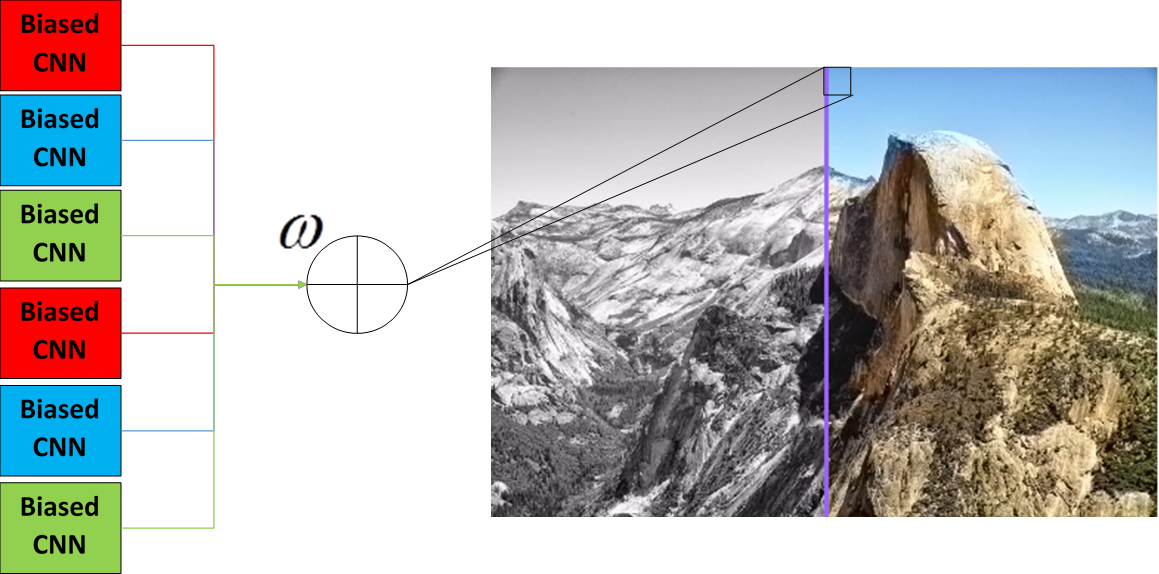
\includegraphics[width=0.45\textwidth]{images/ensemble}
  \textbf{\caption{Architecture of recolorization ensemble}\label{fig:recolor_arch}}
\end{figure}

We propose a novel method for image colorization by boosting the outputs of an ensemble of chromatic biased CNNs to effectively enhance the saturation of the reconstruction. The algorithm is outlined in figure \ref{fig:recolor_arch}. We partition our input dataset into thirds depending on the abundance of pixels containing red, blue or green color components in a given image.

This method of partitioning our dataset is based on the observation that training just a single CNN causes it to average all of the color values to a desaturated sepia tone. We hypothesize that biasing the input dataset in this manner will enhance the saturation of a single channel in the output while causing the other channels to appear desaturated. Combining the outputs of each member of the ensemble by taking a weighted sum on a per pixel basis will then allow us to obtained a more visually appealing image that does not suffer from the desaturation problem that previous approaches face.

\section{Related Work}

A literature study showed us that all modern automatic colorization techniques utilize Convolutional Neural Networks to learn the prediction functions that map from grayscale to color space. However, they differ in the manner in which they model their color space as well as their CNN architecture.

\subsection{Hypercolumns}
Larsson et al.\cite{Larsson2016} recognize that simply using the final layer of the CNN output to represent features causes the system to be unable to precisely localize features in the image. The  intermediate outputs of the neural networks have the ability to provide finer localization but lack the correct semantics to efficiently classify these features.

Larsson et al. successively extract outputs at intermediate layers of the CNN, upscale them to the original size of the image, and concatenate them together. In this manner they create a vector for each pixel. Thus, they feed this hypercolumn\cite{Hariharan2015} - a vector of activations of all CNN units above the given pixel - as a descriptor for each pixel into the fully connected layer in order to obtain precise localization data while preserving representational semantics.

\subsection{Class Rebalancing}
Most automatic colorization methods tend to be biased towards desaturated colors such as beiges and light blues as these colors appear in the greatest frequency in image backgrounds while more saturated colors tend to be comparatively rarer.

Zhang et al.\cite{Zhang2016} work off of the inherent multimodal nature of the colorization problem and first quantize the \textit{ab} output space(chromatic components \textit{Lab} colorspace) into bins after which they generate a distribution of colors at each pixel. They then re-weight the loss of each pixel at train time based on pixel color rarity so as to encourage the network to learn rarer, saturated colors. The final pixel output is then obtained by taking the annealed mean of the pixel distribution.

\subsection{Colornet}
\begin{figure}[ht]
  \centering
    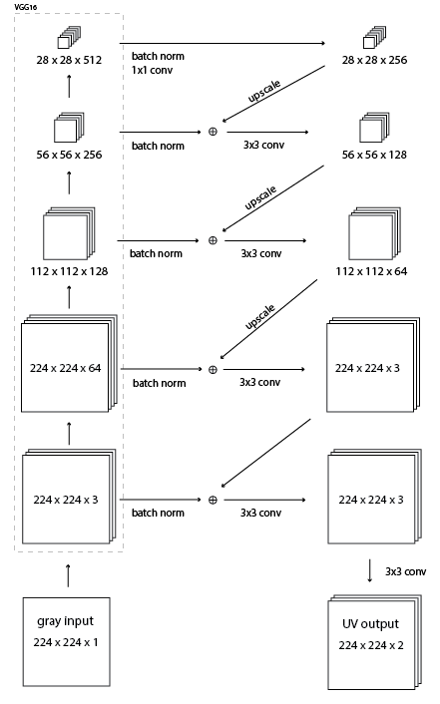
\includegraphics[width=0.25\textwidth]{images/colornet_arch}
  \textbf{\caption{Architecture a single Colornet CNN \cite{ColorNet}}. \label{fig:colornet_arch}}
\end{figure}

\begin{figure*}
  \centering
    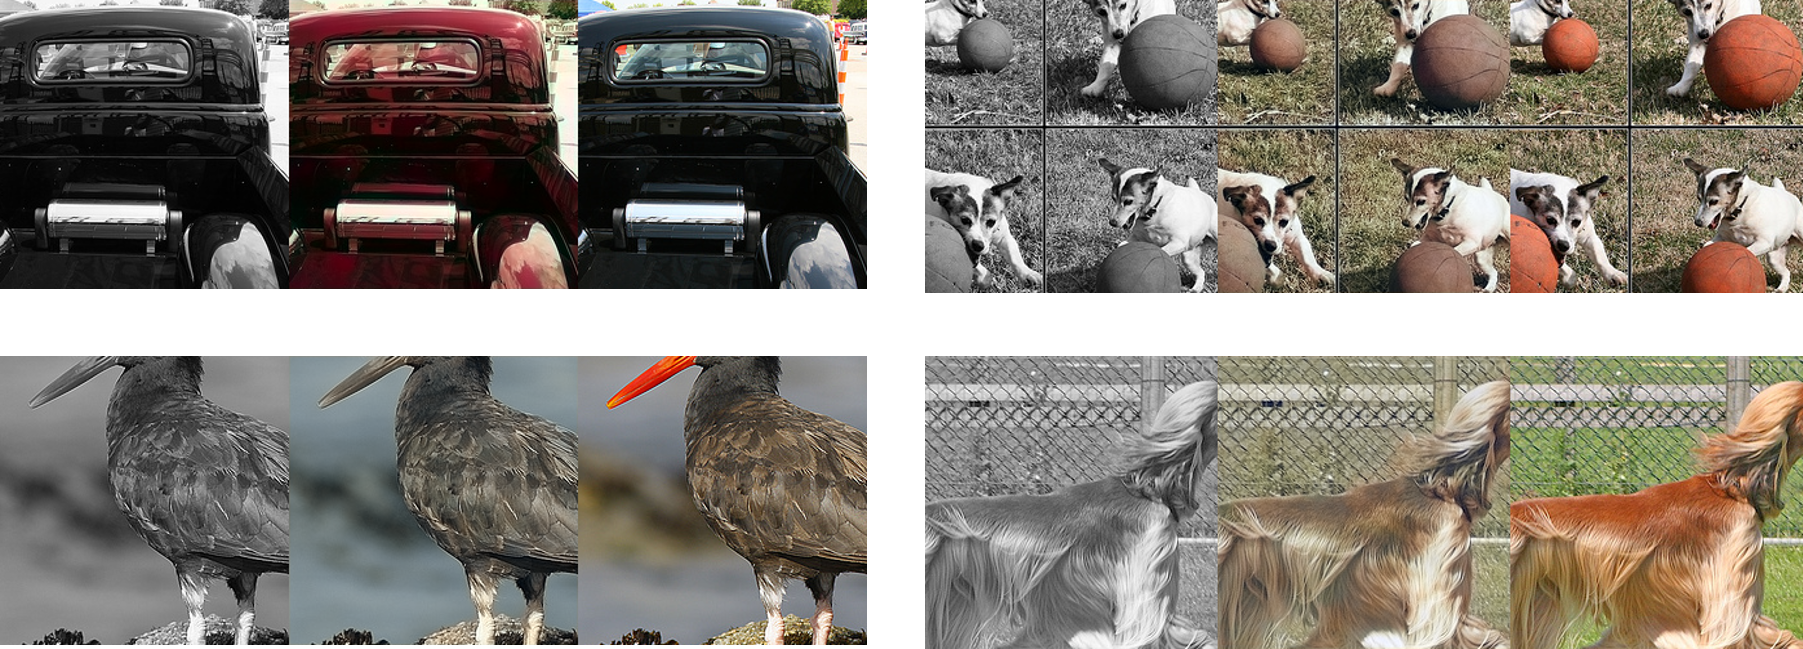
\includegraphics[width=1\textwidth]{images/colornet}
  \textbf{\caption{Colornet colorization results \cite{ColorNet}. Left is the grayscale input, center is the reconstructed image, and right is ground truth. Each image shows high bias. The image on the top left shows a large bias towards red, and the other three images have high desaturation.}\label{fig:colornet_examples}}
\end{figure*}

Colornet is an open source CNN designed to colorize grayscale images implemented using the TensorFlow library\cite{ColorNet}. This network represents the objects in YUV color space and thus maps the luminance Y in grayscale images to the U and V channels \cite{YUVColorSpace}. This model builds off of the VGG16 \cite{VGG16} network, and utilizes hypercolumns as pixel descriptors by extracting the intermediate networks outputs before the first 4 pooling layers, upscaling them to the original image size and then concatenating them.

The network can operate with a simple loss function such as Euclidean distance. However, empirical results showed that the performing this calculation after blurring the input image with a Gaussian kernel allowed the network to converge faster\cite{ColorNet}.

Results for the pretrained model can be seen in figure \ref{fig:colornet_examples}. The results can be seen to get fairly accurate colors in some cases, but the colors are almost always desaturated or washed with a sepia tone. We work to improve the desaturated results of this model by modifying the Colornet project.

\section{Approach and Algorithm}

We use the network structure used by Colornet \cite{ColorNet} in our ensemble. These models will be trained on a subset of the ImageNet database \cite{Russakovsky2015}. This dataset will be partitioned into three sets, each biased towards one of the RGB color channels. A Colornet network will be trained on each of these datasets, leading to three total networks in our ensemble, each of which is biased towards a particular color channel. In the ensemble, the outputs of the networks are combined using a pixel-by-pixel weighting, where the saturation value of the output is used as the confidence, and weights a network's contribution to the output.

\subsection{Dataset}

The networks were tested and trained on a subset of the ImageNet database \cite{Russakovsky2015}. The images were rescaled to 256x256 for consistency, as the Colornet network takes 224x224 random crops of the image during training. We also perform some preprocessing on the dataset. Namely, we remove all grayscale images from the training set, as these images will degrade the quality of the trained models. The cost function for the network is the MSE of the output and original image. Thus, having an abundance of grayscale images will bias the output towards desaturated and grayscale color values.

Additionally, we partition the dataset into three classes of data, one for each of the RGB color channels. Each dataset consists of images that are "mostly" that color, which we will define more concretely in the next section. Then, we train an independent Colornet network on each of these partitions. Doing so creates a CNN that is biased towards that given color.

\subsection{Biased CNN's and Dataset Partitioning}

The issue with automatic colorization networks is that they often generate desaturated images, and the colors tend to be grayish or brownish. The primary reason for this, we hypothesize, is that the network learns the average of all the colors it sees in the images, which leads to the a brownish/grayish tone that washes over the entire image image, as seen in the images in figure \ref{fig:colornet_examples}.

To deal with this issue, we partition our dataset into classes based on which color is most preeminent throughout the image (red, green, or blue), and then train a network on this partition. The idea is that if we constrain images to mostly red, blue, or green the trained network will learn that color channel well, rather than learning the average of the channels. Additionally, since the data is constrained a smaller amount of data should be required to train a good network, and it should converge faster. This generates a CNN that is biased towards a color, effective at detecting that particular color in an image. The three CNN's are used as an ensemble to generate the final predicted image color.

To partition the data, we use equation \ref{eq:color_partition} to decide which bin to place a given image into. We define the dominant color, or most preeminent color in an image, as the color channel with the highest sum. That is, we sum the color channel values for every pixel in the image. The channel with the highest sum is the dominant color, and that's the bin the image is partitioned into.

\begin{equation}
    \underset{c \in \{R, G, B\}}{\arg\max} \sum_x \sum_y I_{xy_c}
    \label{eq:color_partition}
\end{equation}

\subsection{Network Structure}

We use an ensemble of 3 identical CNN's, each biased towards a particular color channel as described in the previous section. These 3 networks' outputs are weighted and combined to generate the final colorized image output. Weighting is done on a pixel-by-pixel basis, which is elaborated upon in the next section. These weights are not learned.

Each network has an identical architecture to the Colornet network \cite{ColorNet}, as shown in figure \ref{fig:colornet_arch}. The Colornet network is in turn based off of the VGG-16 \cite{VGG16} network. Colornet is a residual network that utilizes VGG-16.

\subsection{Recombination Weighting}

\begin{figure}[ht]
  \centering
  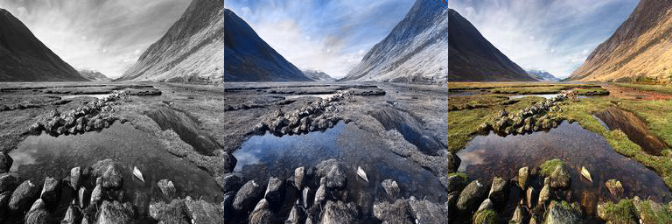
\includegraphics[width=0.45\textwidth]{images/desaturated_blue}
  \textbf{\caption{A CNN trained on blue biased images. It can be seen that the confident areas have accurate colors, and the less confident ones are gray and desaturated. This makes it easy to identify where a particular CNN performs well.}\label{fig:sat_conf}}
\end{figure}

When evaluating images, we need to combine the outputs of each biased CNN into a final result. The strategy we used here was a per-pixel recombination using the saturation value. This is expressed by equation \ref{eq:sat_recomb}. For each pixel in the image, we transform it to HSV color space and look at the saturation values of the $n$ outputs from the CNN's. Each CNN's contribution to the output is weighted by its saturation value over the sum of saturations across the $n$ CNN's. This weights each CNN relative to the other ones based on saturation.

\begin{equation}
    I_{xy} = \sum_{i=1}^n \frac{s_{i_{xy}}}{S_{xy}}I_{i_{xy}}, \qquad S_{xy} = \sum_{i=1}^n s_{i_{xy}}
    \label{eq:sat_recomb}
\end{equation}

The reason that saturation is used is because it represents the confidence of the network when it colors a given pixel. Our goal is to create images with saturated colors, and prevent a bias towards desaturation that other networks suffer from. Thus, we want to prefer CNN outputs that have a high saturation, as this will give images saturated colors.

Figure \ref{fig:sat_conf} demonstrates how saturation correlates with confidence. This image is evaluated using a blue-biased CNN. The sky and water both have highly saturated colors, which is because the CNN has seen many skies and bodies of water in its training set. The landscape, however, is typically not blue, so the CNN is less confident in its prediction, leading to a desaturated and more grayish color for its prediction. It is for this reason that we use saturation as the weighting value for when we combine the results of the biased CNN's.

\subsection{Hardware and Software Stack}

The ensemble colorization system is very computationally expensive. VGG-16 is a large network with too many parameters to be trained in reasonable time from scratch on regular CPUs. Thus, we had to train on with a GPU to ensure that training would complete in a reasonable amount of time. A desktop with an NVIDIA 980Ti GPU was used to perform training. The training is accelerated using cuDNN, with the Tensorflow library acting as the middle layer between our code and the GPU driver.

As mentioned before, we based our network off of Colornet \cite{ColorNet}, so we utilized their python code as a starting point for our design. Using TensorFlow greatly minimized our implementation and debugging time. Both of these allowed us to quickly start adding our own features to the exiting code.

Since we use TensorFlow, we also wrote our entire preprocessing and data augmentation pipeline in Python. This made it very easy to quickly prototype and modify hyperparameter settings for the system. Also, it allowed us to use many existing Python libraries for data augmentation and image processing. The pixel-by-pixel recombination was written in Python, utilizing NumPy, also allowing for this to be easily tested and updated.

\section{Results}

\subsection{Data Partition Results}

We first train networks on partitions of the training dataset and analyze the results separately. Here we can see examples from three of the resulting CNNs. These CNNs were trained on approximately 10 epochs of around 50k images for blue and green, and 150k images for red (red images are far more prevalent in the training set used than blue or green). The results show areas each type of CNN is particularly successful at. It can be seen in some images, such as the woman in figure \ref{fig:res_green_biased}, that gray washed areas are areas about which that the network is not confident.

\begin{figure}
  \centering
    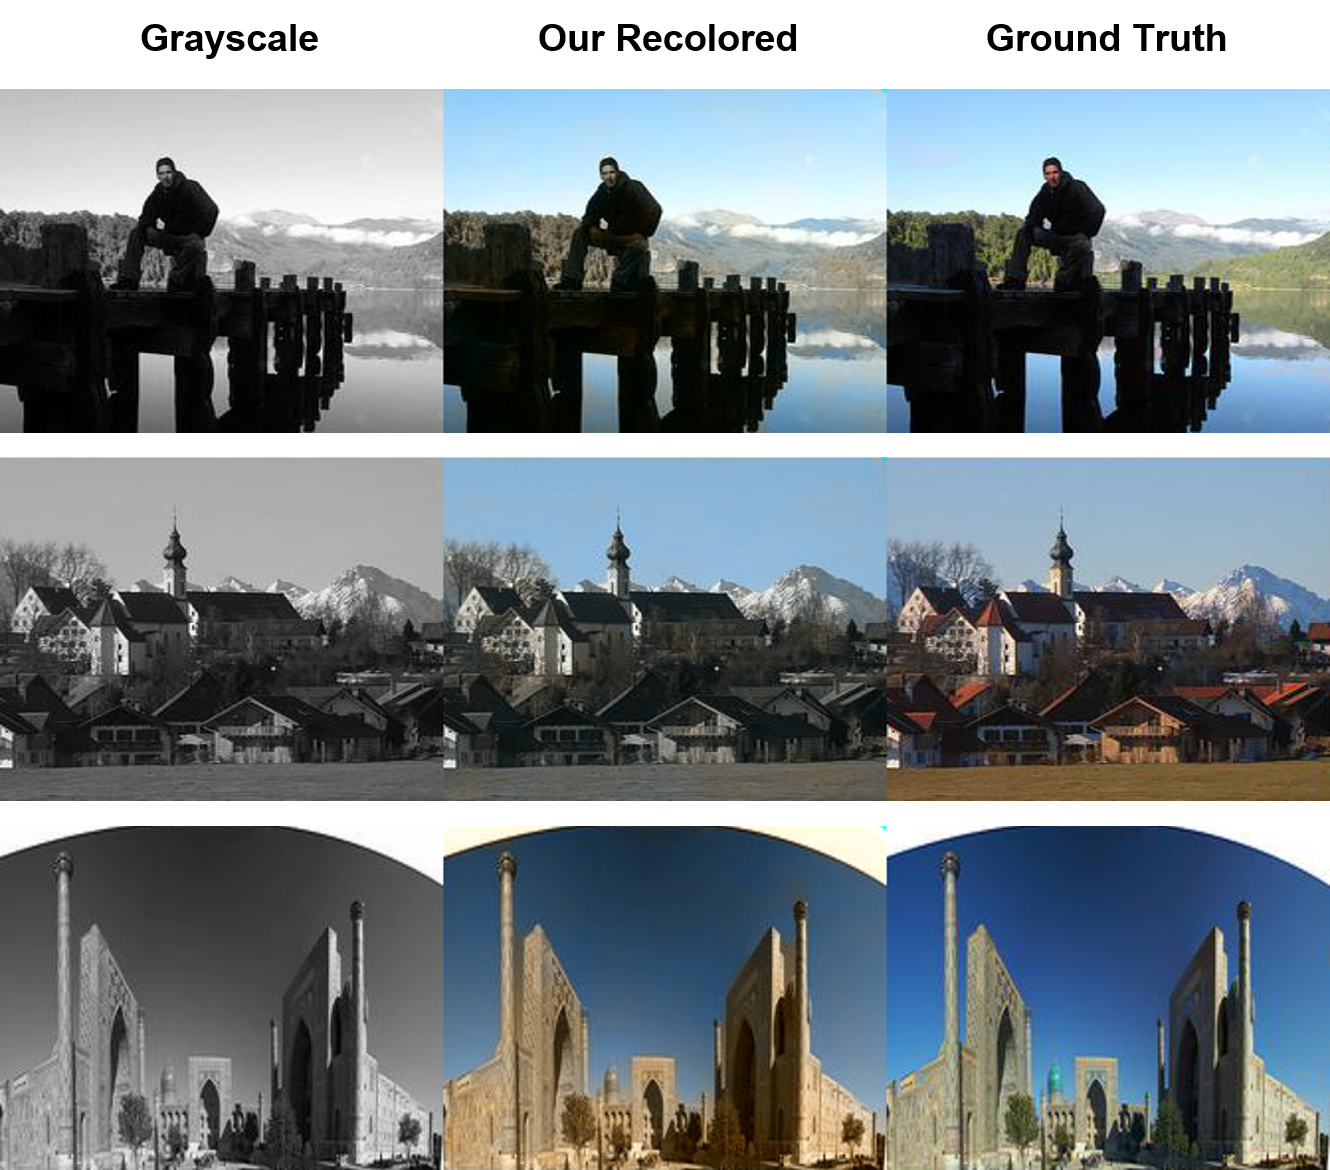
\includegraphics[width=0.45\textwidth]{images/blue_bias}
  \textbf{\caption{CNN Biased towards blue images: trained only on images that had strong blue components. Note that all the resulting images are strong in areas such as sky, water, and atmosphere effects, but are weak in houses, buildings, and human skin.}\label{fig:res_blue_biased}}
\end{figure}

\begin{figure}
  \centering
    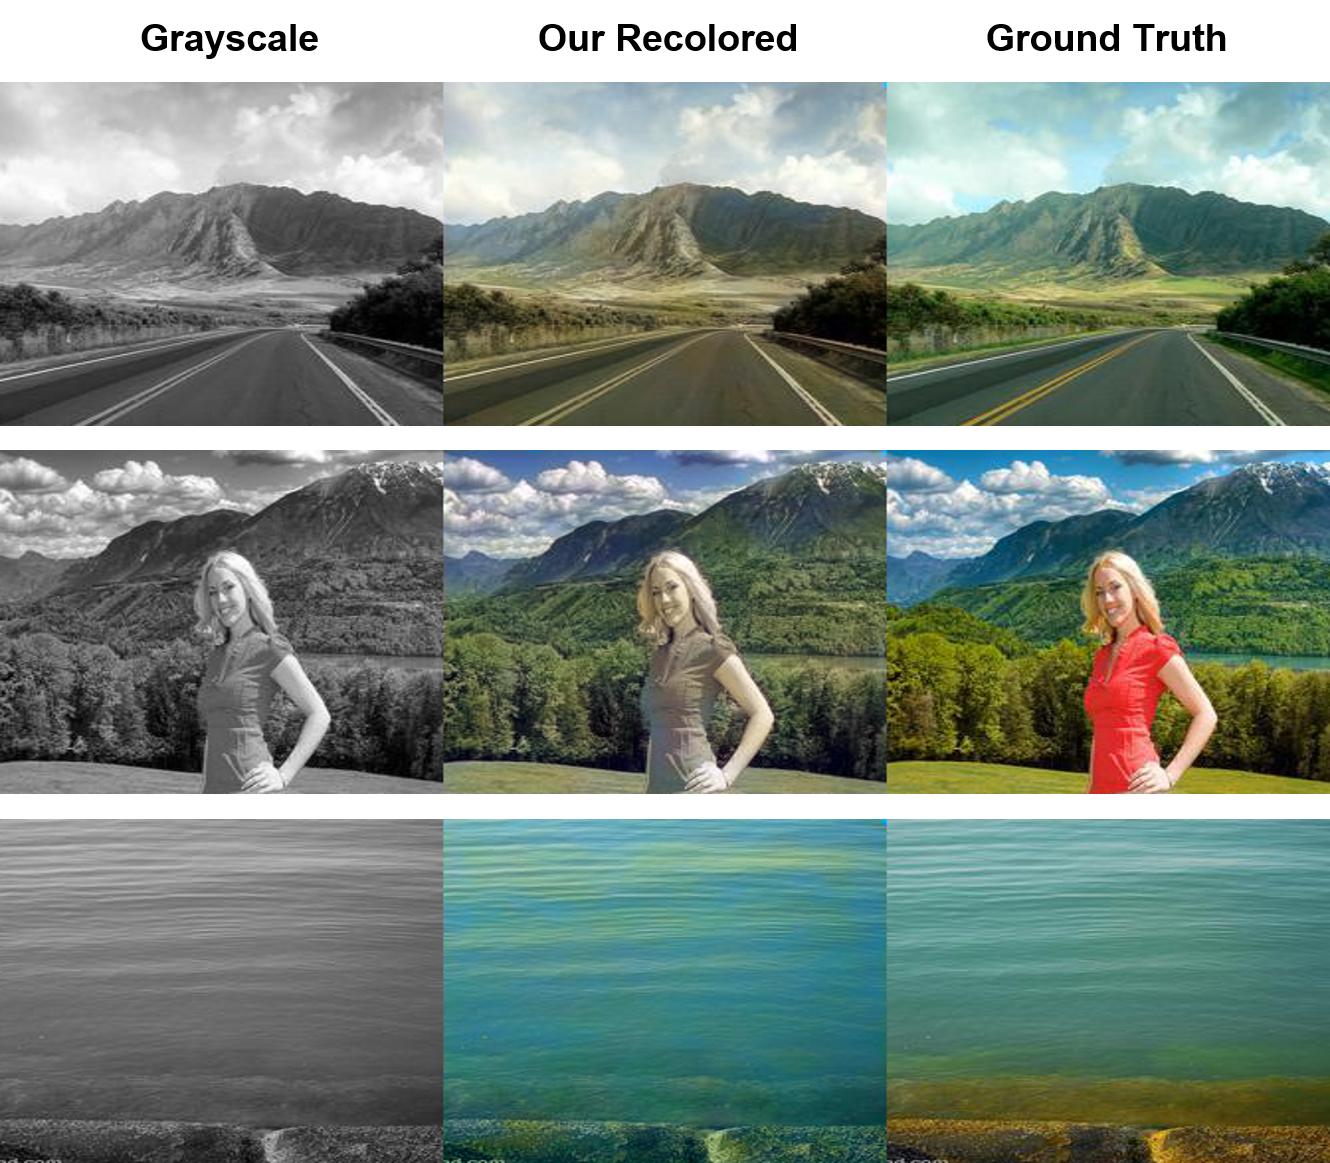
\includegraphics[width=0.45\textwidth]{images/green_bias}
  \textbf{\caption{CNN Biased towards green images: trained only on images that had strong blue components. This CNN is particularly good at landscapes and grass.}\label{fig:res_green_biased}}
\end{figure}

\begin{figure}
  \centering
    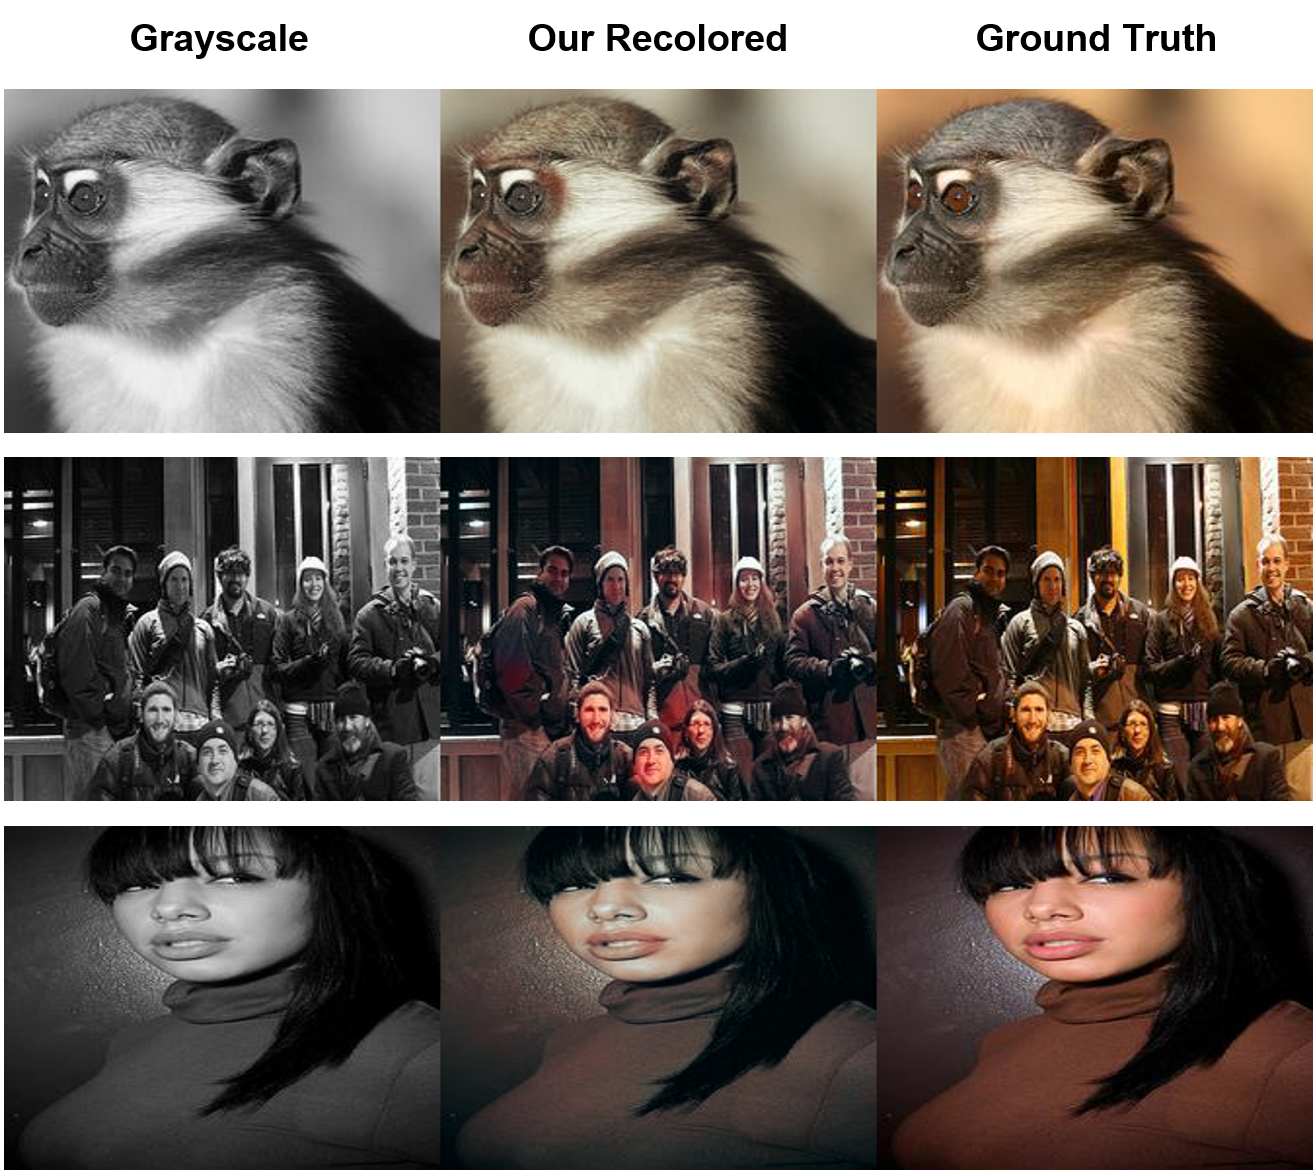
\includegraphics[width=0.45\textwidth]{images/red_bias}
  \textbf{\caption{CNN Biased towards red images: trained only on images that had strong blue components. This CNN is strong in areas of humans and animals, clothes, faces, and common red objects with strong patterns such as brick.}\label{fig:res_red_biased}}
\end{figure}

\subsection{Per-pixel Weighted Recombined Results}

Here, in figure \ref{fig:res_recombined}, we show the results on an image of recombination by per-pixel reweighting. Each of first three biased images predict different areas of the image well and with believable colors. However, each one fails at a different area. In the recombined version, the sky has high weighting from the blue CNN, and the green and red CNNs help define the building texture. Note the red in the clouds is likely from training on a lot of sunset type scenes. Success seems to vary across image types. Images that naturally are saturated see more success from this method, but images that are naturally desaturated can show high bias.

\begin{figure}
  \centering
    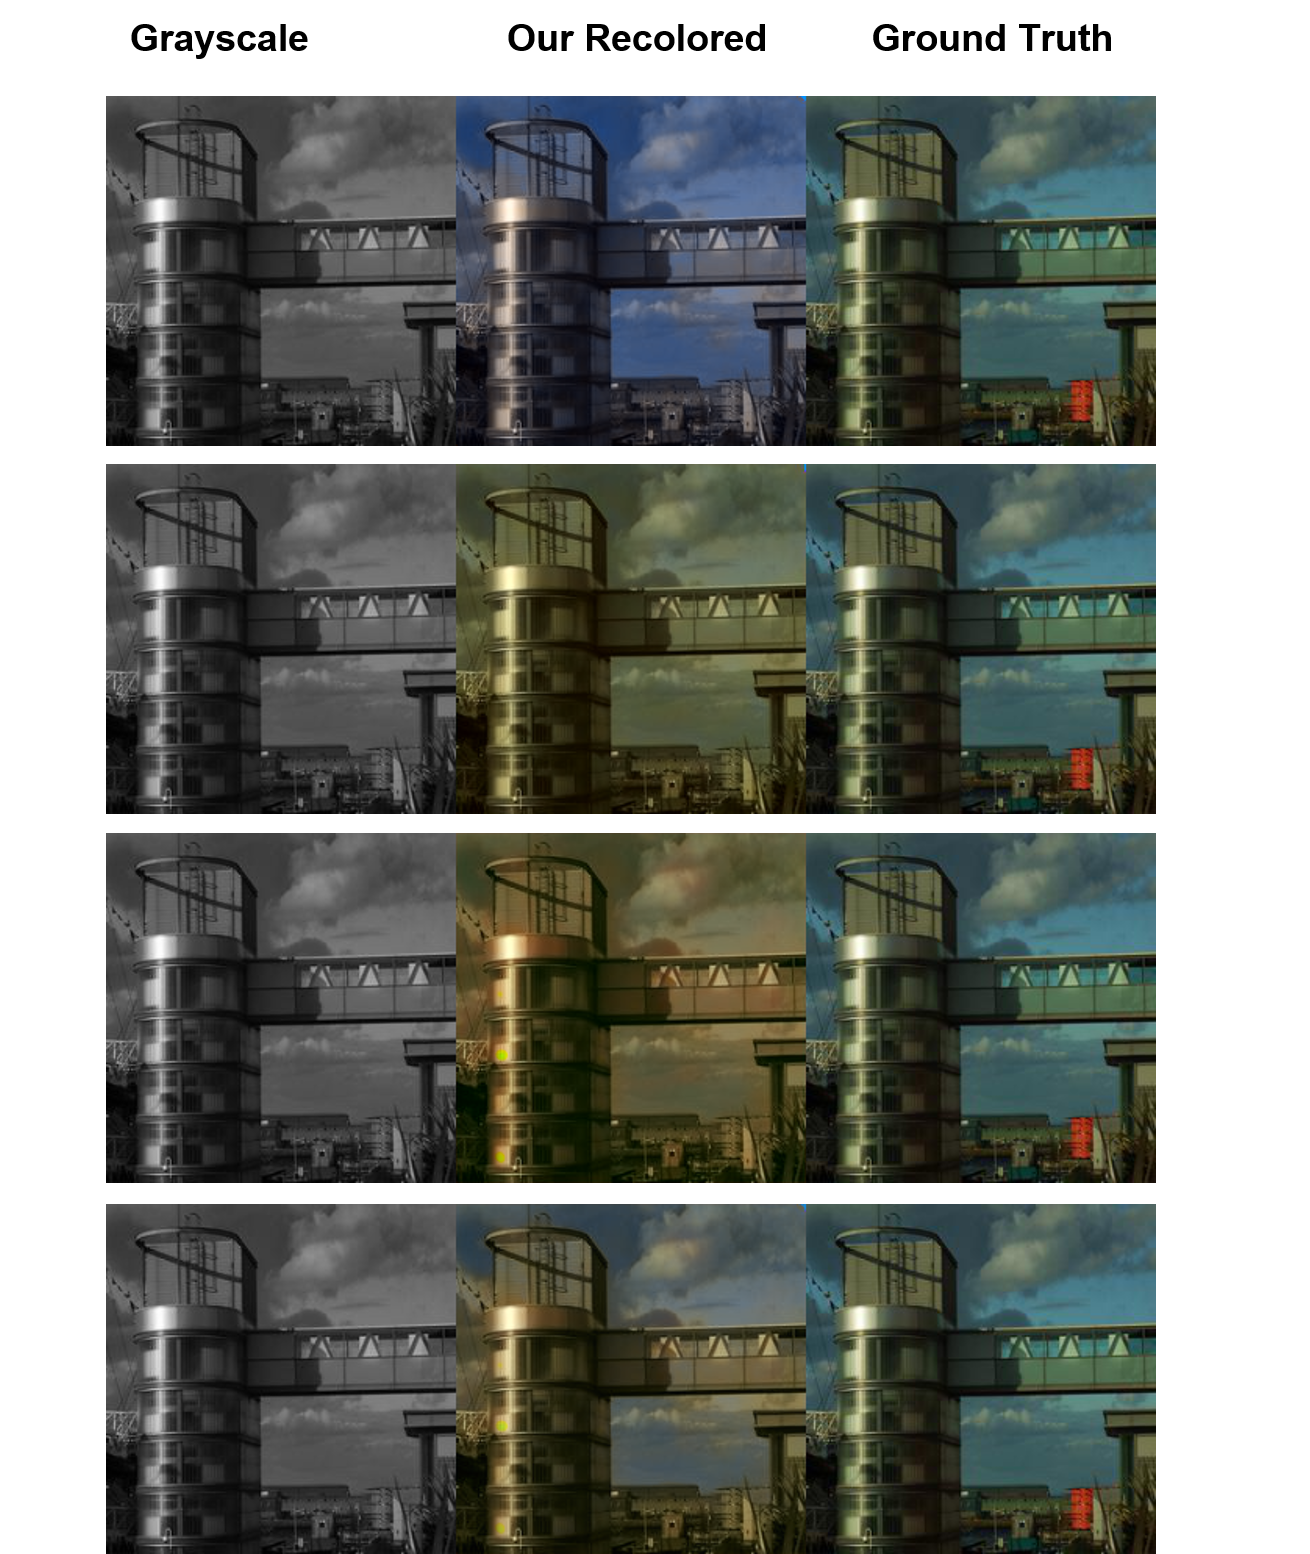
\includegraphics[width=0.5\textwidth]{images/recombined}
  \textbf{\caption{From top to bottom: Biased towards blue, green, and red. Last is combined based on weighted saturation per pixel. Note that recombined version has best parts of all three images and does not lose saturation and get washed with sepia.}\label{fig:res_recombined}}
\end{figure}

\section{Conclusions}
In this paper, we have presented an automatic grayscale image colorization system that attempts to enhance the saturation of the output image by leveraging an ensemble of chromatic biased CNNs. Two novel contributions make this model effective. First, partitioning the input datasets based on relative abundance of components prevents the networks from averaging the outputs into a desaturated sepia tone. Second, combining saturation of outputs on a per pixel basis allows us to augment high confidence network outputs while suppressing desaturated and low confidence outputs.

Our results indicate that while the output of our ensemble is at times very different from the the actual colored images, it produces  plausible colorized versions of the input grayscale images that are more visually appealing that those produced by the standalone Colornet implementation.

\section{Future Work}
An advantage of our proposed model is that it is easily extensible. In this paper, we focused our efforts on using CNN biased towards either red, green or blue components. However, future studies could examine the efficacy of color spaces such as \textit{Lab}, YUV, or HSV. In addition, studies could also examine whether permutations of CNNs biased towards different color spaces could produce better output images compared to a set of CNNs biased towards a single color space.

The optimizer used in each of the individual CNNs also provides an additional opportunity for future exploration. Our implementation used a gradient descent optimizer which can get stuck in local minima. This is a definite possibility given the under-constrained nature of the colorization problem. Using an optimizer with momentum as an additional hyperparameter could result in greater saturation for the output image

{\small
    \bibliographystyle{ieee}
    \bibliography{references}
}
\end{document}
